\documentclass{article}
\usepackage{amsmath}
\usepackage{amssymb}
\usepackage{amsthm}
\usepackage{float}
\usepackage{graphicx}
\usepackage[includefoot, bottom=12pt]{geometry}
\usepackage{hyperref}
\usepackage{subcaption}
\usepackage{fancyhdr}
\usepackage{listings}
\usepackage{bbm}

\geometry{left=1.25in}

\pagestyle{fancy}
\graphicspath{{./}}
% \fancyhead{}
% \fancyfoot{}

\fancyhead[R]{Neeraje,  Balaji,  Moulik}
\fancyhead[L]{\leftmark}

\renewcommand{\sectionmark}[1]{\markboth{#1}{}}

\title{DAI Assignment-3}

\author{Aditya Neeraje,  Balaji Karedla,  Moulik Jindal}

\date{\today}

\begin{document}

\maketitle
\tableofcontents

\pagenumbering{gobble}

\newpage

\pagenumbering{arabic}
\section{Question 2}
\subsection{Part 1}
\subsubsection{Part b: }
\lq\lq I want you to continue this time series and forecast the next 8 values. There is seasonal periodicity with period 12,  but due to Covid,  there is a huge dip in the middle. Thus,  more recent values will be more relevant: \lq1408012, 1341210, 1423569, 1511094, 1685168, 1480879, 1445248, 1531406, 1378691, 1510184, 1467763, 1575872, 1426580, 1464070, 1601141, 1679963, 1908334, 1797101, 1599977, 1858664, 1907378, 1890273, 1967992, 2324221, 2276404, 2230645, 2286128, 2481285, 2769283, 2536554, 2416916, 2384943, 2430449, 2589861, 2597765, 2743325, 2725711, 2754131, 3023228, 3066556, 3336839, 3023081, 3383768, 3341081, 3295826, 3692828, 3772583, 3848322, 3809228, 3418605, 3611371, 3778780, 4190914, 3825814, 3699451, 3678245, 3664509, 4133027, 4131844, 4430070, 4556904, 4290189, 4576236, 4579916, 4852909, 4672686, 5002416, 4757378, 4920335, 5074853, 5005919, 5478523, 5321832, 4930608, 5440796, 5481088, 5979551, 5778376, 5693448, 5540693, 5559031, 5842318, 6151347, 6188457, 6119924, 5931189, 3793464, 1967859, 142254, 1046836, 1272240, 1681787, 2265539, 2926835, 3423059, 3951522, 4202712, 4238466, 4184920, 3083318, 1168738, 1701955, 2932469, 3816286, 3958375, 4807415, 5706021, 6140654, 3556558, 3950597, 5783838, 5957411, 6376429, 5982787, 5711288, 5832025, 5972449, 6471441, 6500903, 6997472\rq\rq\rq
I gave this prompt to ChatGPT,  and it gave the following response:\\
\begin{figure}[H]
\centering
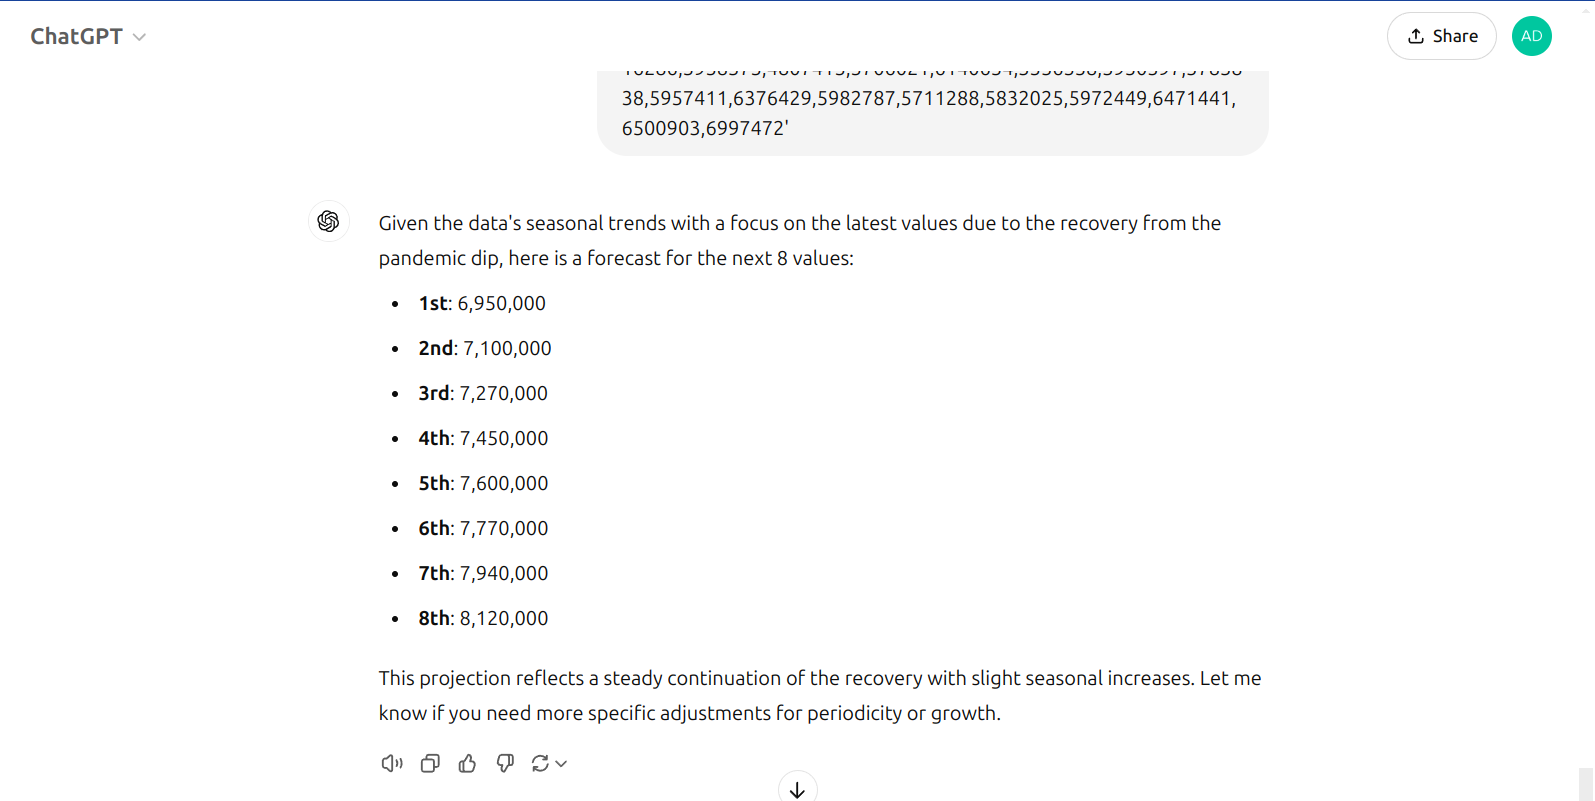
\includegraphics[width=\textwidth]{ChatGPT Response.png}
\end{figure}
The mean\_absolute\_percentage error is 2.81\% for these predictions (Jan-July 2023).
\subsubsection{Part c: }
For the forecasting,  we used a VARIMA model from u8darts. After some testing, values of p=2,d=1,q=2 and a trend which fits a linear polynomial in terms of time gave us our best results,  with an MAPE of 4.8\% between January and August 2023. 
\subsection{Part 2}
MAPE penalizes overprediction more than underprediction since it is unbounded for overpredictions while MAPE is normally small for underpredictions as it is bounded by 100\%. Using MAPE as a metric often results in the forecast being conservative in its estimate. However,  for an airline,  because of the immense logistical difficulty of buying new aircraft,  underprediction of demand leads to significantly more loss,  whereas if there are aircraft having a few free seats,  some cost can still be recovered by offering these seats at discounted prices to ensure all seats will be full,  or my adding new routes/destinations with the extra aircraft/personnel.\\
Secondly,  MAPE gives high priority to erroneous forecasts on days of low demand. For instance,  on a day with an actual demand of 50,  the model predicted a demand of 100,  versus on a day with an actual demand of 100,  the model predicted a value of 50,  the former would contribute a lot more to the average percentage error than on the latter,  but mispredictions of the peak is worse for the company,  as that would mean it does not have spare capability present on the peak day.\\
WAPE (Weighted Average Percentage Error) would be a better metric. It measures the error as the sum of all absolute errors divided by the sum of absolute values of the datapoints.
\subsubsection{Part 2}
I would use a t-test on the means and variances of the two time periods in the new time series created by considering the difference terms. The null hypothesis would be that the means of the two time series are equal. If the p-value is less than 0.05 or the t-statistic is significant (greater than 2 seems to be the rule of thumb for this,  I think),  we can reject the null hypothesis and conclude that the means of the two time series are different.
\end{document}